\section{Architektur}

Convolutional Neural Network, kurz CNN bzw. ConvNet ist eine Untergruppe von Artificial Neural Network (ANN),  die sich auf die Klassifizierung von Daten gitterartiger Topologie wie Bilder spezialisiert. Wie das menschliche Gehirn kann CNN eine riesige Menge an Daten aus einem Bild extrahieren und verarbeiten, weshalb es zur Modellierung des menschlichen Sehens von Bedeutung ist. 

In den folgenden Unterabschnitten wird die allgemeine Architektur eines CNNs (\ref{CNN}), die logistische Regression zur Klassifikation binärer Zielvariablen im CNN (\ref{subsec:logReg}) und das EfficientNet als final gewählte Architektur (\ref{EfficientNet}) erklärt; englische Fachbegriffe werden im Verlauf bewusst beibehalten und nicht ins Deutsche übersetzt, um Präzision zu verleihen.

% ----------------------------
\subsection{CNN} \label{CNN}
% ----------------------------
CNN umfasst eine Klasse von Architekturen, die sich in der Anzahl der Layers, Anzahl der Filter, Filtergröße usw. unterscheiden. Dennoch ist jedes CNN hauptsächlich gekennzeichnet durch drei Layer: Convolutional Layer, Pooling Layer und Fully Connected Layer. Die ersten beiden Layer dienen zur Feature Extraction und Feature Learning und die letzte Layer ist verantwortlich für die eigentliche Klassifizierung. Eine Layer besteht dabei aus einer Sammlung von Neuronen und besitzt ihre eigenen Gewichten und Biases.


\begin{figure}[H]
\centering
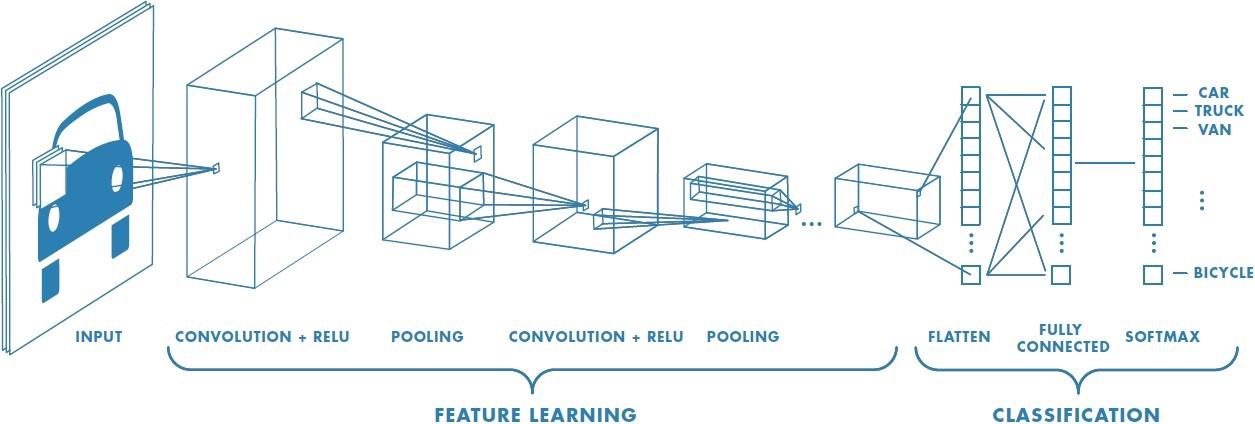
\includegraphics[width=0.8\linewidth]{pic/Klassifikation/CNN-Architektur.jpeg}
\caption{\label{pic:cnn} CNN Architektur}
\end{figure}



Nachfolgend werden die verschiedenen Layers eines allgemeinen CNNs, wie in der obigen Abbildung gezeigt, erläutert und anschließend der Trainingsalgorithmus eines CNNs präsentiert.
Die Arbeiten in \cite{1}, \cite{2}, \cite{3}, \cite{4} und \cite{5} dienen dabei als Grundlage für die nachstehende Darlegungen.

\subsubsection{Input}
Jedes Eingabebild wird durch eine Matrix bzw. Matrizen von Pixelwerten, auch als Tensor bezeichnet, repräsentiert. Es wird dabei zwischen einem farbigen, einem Graustufen bzw. einem Schwarz-Weiß-Bild unterschieden. Ein farbiges Bild wird durch drei Farbkanäle: rot, grün und blau, gekennzeichnet, wobei die Kanäle als 2D-Matrizen mit Pixelwerten zwischen 0 und 255 dargestellt werden. Weniger Speicherbedarf hat ein Graustufen-Bild, da dieses durch eine einzige 2D-Matrix, ebenfalls mit Pixelwerte zwischen 0 und 255, beschrieben wird. Noch weniger Speicher benötigt ein Schwarz-Weiß-Bild, welches nur Pixelwerte von 0 und 1 enthält. 

\subsubsection{Convolutional Layer} 
Das Eingabebild wird nun in die Convolutional Layer weitergegeben, in der dessen wesentliche Informationen (Features) extrahiert werden; man spricht hierbei von Feature Extraction. 

Die Convolutional Layer ist Kernbestandteil des CNNs und trägt den Hauptteil der Rechenlast des Netzwerkes. Sie  besteht aus linearen (Convolution) und nichtlinearen (ReLU) Operationen. Lineare bzw. Convolution Operationen sind für das eigentliche Feature Extraction verantwortlich, während nichtlineare Operationen schließlich angewendet werden, um der Rechenaufwand, vor allem in der Backpropagation, zu verringern.

Das Feature Extraction in der Convolution erfolgt durch die Matrixmultiplikation von zwei Matrizen; die eine ist der sogenannte Kernel und die andere ist das rezeptive Feld des Tensors, welche sich durch das Schieben über die Höhe und Breite des Tensors ergibt. In der unteren Abbildung \ref{pic:convolution} entspricht das rezeptive Feld dem orange-markierten Bereich im Input Tensor.

\begin{figure}[H]
\makebox[\linewidth]{%
  \begin{tabular}{ccc}
    &  &  \\
    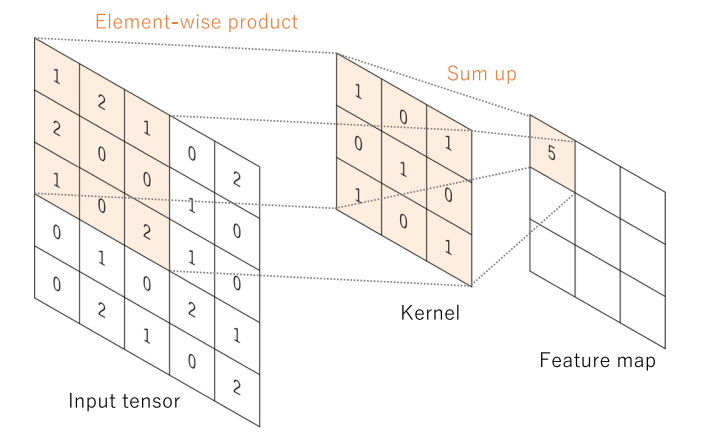
\includegraphics[width=0.28\linewidth]{pic/Klassifikation/convolution1.png}&
    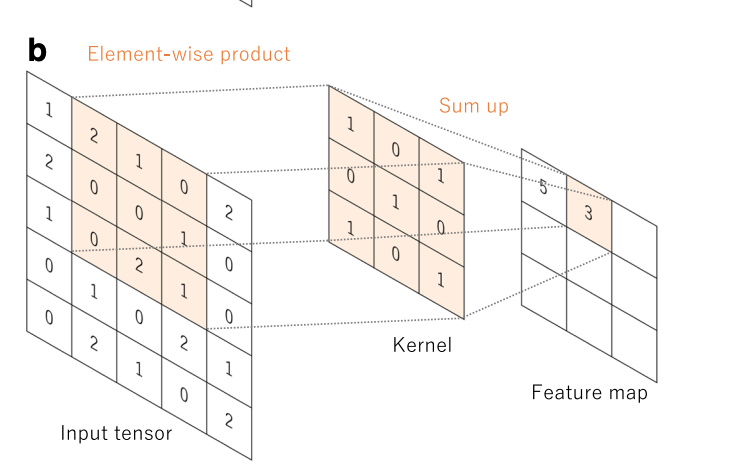
\includegraphics[width=0.28\linewidth]{pic/Klassifikation/convolution2.png}&
    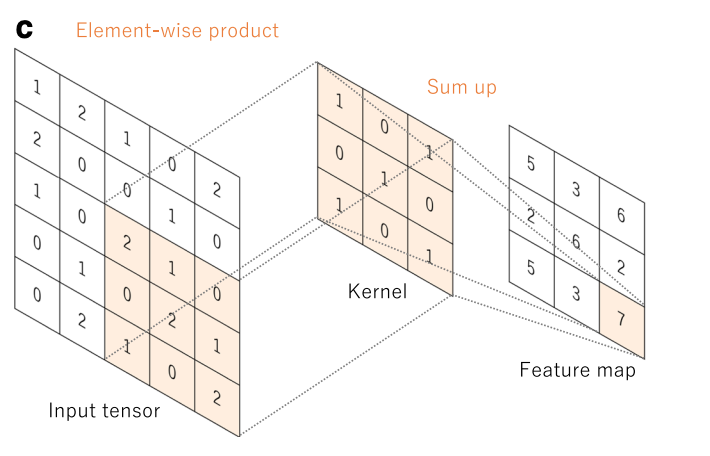
\includegraphics[width=0.28\linewidth]{pic/Klassifikation/convolution3.png}\\
  \end{tabular}%
}
 \caption{Convolution mit einem 3$\times$3-Kernel und Stride=1}
  \label{pic:convolution}
\end{figure}


Der Kernel ist in der Regel eine 3$\times$3, manchmal auch 5$\times$5 oder 7$\times$7 Matrix. Welche Features aus dem Tensor extrahiert werden, wird mit der Wahl der Kernels entschieden. Je mehr Kernels für die Convolution gewählt wird, desto mehr Informationen werden erfasst. Es ist jedoch anzumerken, dass mit der Genauigkeit auch die Rechenlast des Netzes ansteigt.


Die sich aus der Matrixmultiplikation ergebende Matrix heißt Feature Map. Ihre Größe wird durch drei Parameter bestimmt: Anzahl der Kernels, Stride und Padding (siehe \ref{def:FeatureMapDimCL}). Dabei gibt der Stride an, um wie viele Einheiten der Kernel über den Tensor vor jeder Matrixmultiplikation geschoben wird. Das Padding beschreibt das Auffüllen von Werte wie z.B Nullen (Zero-Padding) um den Tensor-Rand herum, um Informationsverlust zu vermeiden. Mit der Verwendung eines Zero-Paddings wird Convolution auch Wide Convolution genannt, während Narrow Convolution eine Convolution ohne Zero-Padding beschreibt.

\begin{Definition}[Dimension der Feature Map im Convolutional Layer] \label{def:FeatureMapDimCL}
Es seien ein Tensor der Dimension $n$$\times$$n$ und ein Kernel der Dimension $f$$\times$$f$ mit jeweils $p$ die Anzahl der Zerro-Padding Layers, $s$ die Größe des Strides und $z$ die Anzahl der Kernels gegeben, dann ist die Dimension der Feature Map im Convolutional Layer $m$$\times$$m$ gegeben durch: 
\begin{equation}
m \times m = (\frac{n+2p-f}{s} + 1) \times (\frac{n+2p-f}{s} + 1) \times z. \label{Dimension Feature Map im Convolutional Layer}
\end{equation}
\end{Definition}

Mit einer Aktivierungsfunktion werden die Werte der Feature Map nun auf einen bestimmten Bereich transformiert. ReLU ist aufgrund ihrer Performanz die meist verwendete Aktivierungsfunktion in der Hidden Layer von CNNs. Nach einer ReLU enthält die Feature Map nur positive Werte, da negative Werte jeweils durch eine Null ersetzt werden. Eine ReLU Aktivierungsfunktion sieht folgendermaßen aus.

\begin{figure}[H]
\centering
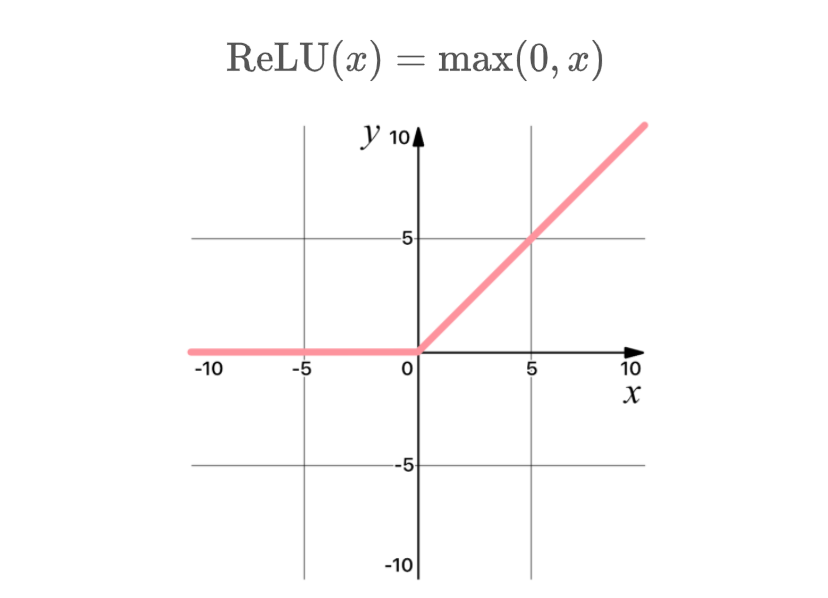
\includegraphics[width=0.5\linewidth]{pic/Klassifikation/ReLU.png}
\caption{\label{pic:ReLU} ReLU Aktivierungsfunktion}
\end{figure}

\subsubsection{Pooling Layer}
Die Feature Map aus der Convolutional Layer wird nun in die Pooling Layer zum weiteren Feature Extraction weitergeleitet. Mit dem Feature Extraction wird die Dimension der Feature Map reduziert und das Overfitting vermieden. Das Netz ist demnach invariant zu kleinen Transformationen,  Verzerrungen und Übersetzungen im Eingabebild. So können Objekte z.B. unabhängig von ihrer Lage im Bild richtig klassifiziert werden. Es gibt verschiedene Arten von Pooling, z.B. Max, Average oder Sum Pooling. In der Praxis zeigt sich das Max Pooling als performanter, weshalb es auch die meist verwendete Pooling Art ist.

Das Pooling funktioniert ähnlich wie die lineare Operation in der Convolutional Layer; auch hier wird ein Kernel über die Eingabematrix geschoben. Nur in der Berechnung der Ausgabewerte gibt es zur Convolutional Layer einen Unterschied. In jedem rezeptiven Feld der Eingabematrix entnimmt der Kernel, je nach Pooling Art, entweder das Maximum, das arithmetische Mittel oder die Summe der Werte des rezeptiven Feldes. Im Fall eines Max Poolings ergeben die Maxima der rezeptiven Felder die Ausgabematrix. Dies wird mit der unteren Abbildung \ref{pic:MaxPooling} veranschaulicht.

\begin{figure}[H]
\centering
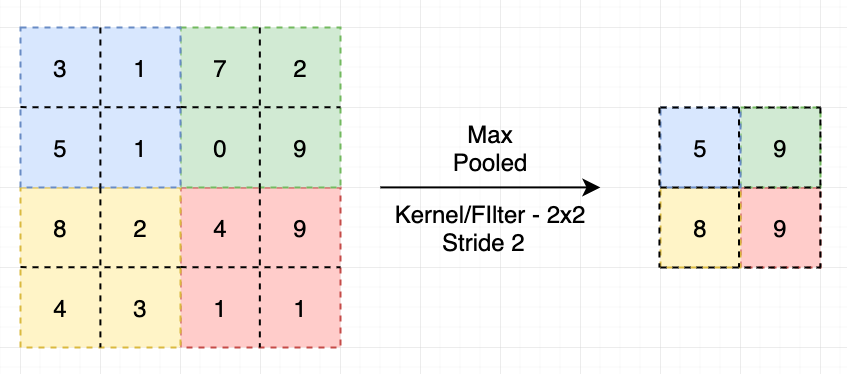
\includegraphics[width=0.5\linewidth]{pic/Klassifikation/MaxPooling.png}
\caption{\label{pic:MaxPooling} Max Pooling mit einem 2$\times$2-Kernel und Stride=2}
\end{figure}

Es gibt in der Regel kein Padding in der Pooling Layer. Die Ausgabematrix wird somit nur von der Dimension der Feature Map und der Größe des Strides beeinflusst. Die Dimension der Feature Map lässt sich, wie in \ref{def:DimFeatureMapPL} definiert, bestimmen.

\begin{Definition}[Dimension der Feature Map im Pooling Layer] \label{def:DimFeatureMapPL}
Es seien eine $n_{H}$$\times$$n_{W}$$\times$$n_{C}$ Eingabematrix (Feature Map nach Convolutional Layer) und ein $f$$\times$$f$ Kernel mit $s$ die Größe des Strides gegeben, dann ist die Dimension der Feature Map $m$$\times$$m$ im Pooling Layer  definiert mit: 
\begin{equation}
m_{H}\times m_{W}\times m_{C} =  (\frac{n_{H}-f}{s} + 1) \times (\frac{n_{W}-f}{s} + 1) \times n_{C}. \label{Dimension Feature Map im Pooling Layer}
\end{equation}
\end{Definition}

\subsubsection{Fully Connected Layer}
Die Feature Map aus der letzten Pooling Layer wird nun transformiert in einen eindimensionalen Vektor (man spricht hierbei auch von Flatten) und in die Fully Connected Layer übergeben. Die Fully Connected Layer ist selbst ein Neuronales Netz, dessen Architektur nach Fragestellung variiert.

Für eine Klassifikation mit binären Zielvariablen eignet sich die Logistische Regression, auf dessen Architektur im Abschnitt \ref{subsec:logReg} eingegangen wird. 

\subsubsection{Der CNN-Algorithmus}
Der Algorithmus des CNN lässt sich nach \cite{2} in fünf Schritten zusammenfassen:
\begin{enumerate}
\item Initialisiere Parameter, Gewichte und Kernels mit zufälligen Werten.
\item Folge der Forward Propagation durch alle Layers der Feature Extraction (Convolution + ReLU, Pooling Layer) in die Klassifikation (Fully Connected Layer) und berechne die ersten Klassenwahrscheinlichkeiten für jedes Objekt.
\item Berechne den Gesamtfehler der Wahrscheinlichkeiten mit:
\begin{equation}
Total Error = \sum \nicefrac{1}{2} (Target Probability - Output Probability) ^2. \label{Total Error}
\end{equation}
\item Folge der Back Propagation und berechne mit dem Gradientenverfahren die neuen, optimierten Parameter-, Gewichten- und Kernels-Werte.
\item Wiederhole die Schritte 2-4 für alle Bilder im Traning Set.
\end{enumerate}


% ----------------------------
\subsection{Logistische Regression} \label{subsec:logReg}
% ----------------------------
Das Konzept der Fully Connected Layer und der Optimierung der Parameter mittels Gradientenverfahren wird in diesem Unterabschnitt an der Logistischen Regression in Anlehnung an der Arbeit von Daniel Jurafsky und James H. Martin (s. \cite{6}) erklärt.



Im Wesentlichen kann die Architektur einer logistischen Funktion anhand von 4 Komponenten beschrieben werden: Feature Vektor, Aktivierungsfunktion (Sigmoid), Verlustfunktion (Cross-Entropy) und Optimierungsalgorithmus (Gradientenverfahren). Diese Komponenten werden im Folgenden genauer erläutert. 


\begin{figure}[H]
\centering
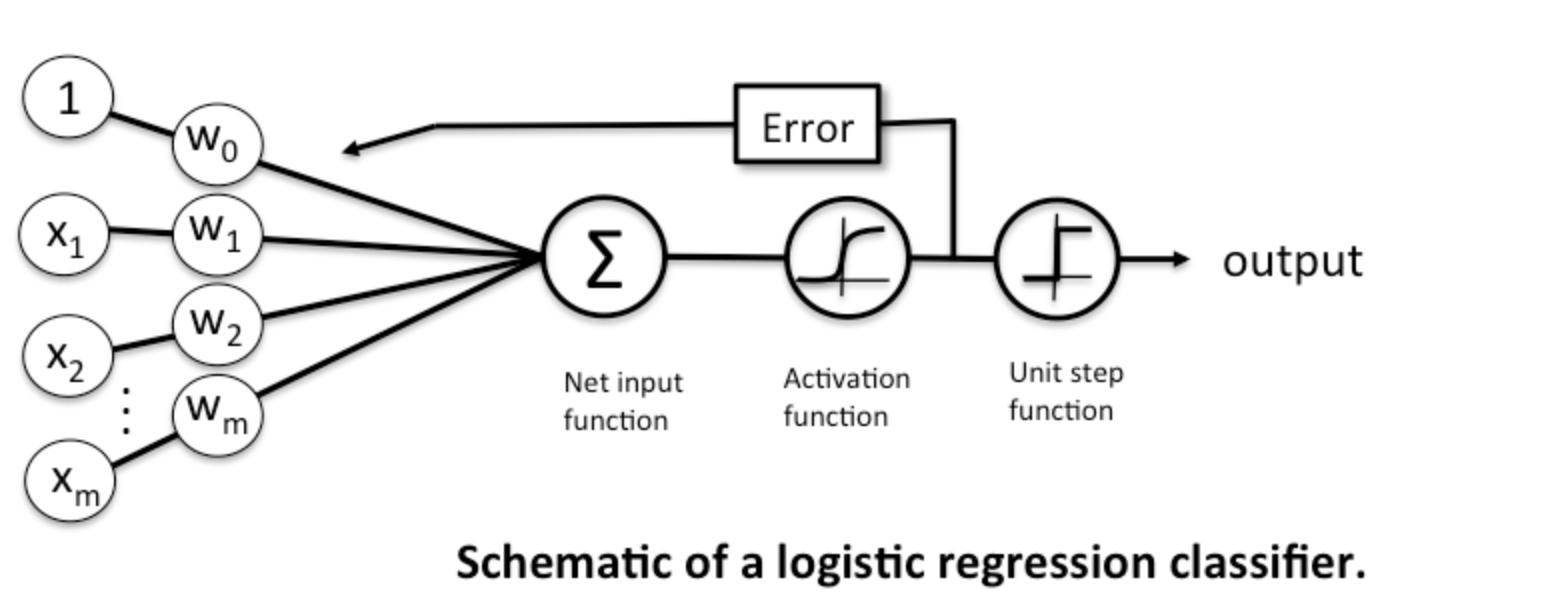
\includegraphics[width=0.5\linewidth]{pic/Klassifikation/LogRegSchema.png}
\caption{\label{pic:logreg} Logistische Regression}
\end{figure}



\subsubsection{Feature-Vektor}
Der eindimensionale Feature-Vektor [ $x_{1}$, $x_{2}$, ..., $x_{n}$ ], der durch das Flatten der Feature Map aus der letzten Pooling Layer entsteht, ist Input der Fully Connected Layer. 
Da jede Klasse von anderen Features charakterisiert wird, ist es von Bedeutung die Features entsprechend zu gewichten. Wir bezeichnen $z$ als die Multiplikation des Feature-Vektors mit dem Gewichten-Vektor [ $w_{1}$, $w_{2}$, ..., $w_{n}$ ] und anschließende Addition mit dem Bias $b$.
\begin{equation}
z = ( \sum\limits_{i=1}^{n} (w_i\cdot x_i)+b ). \label{z}
\end{equation}
Aufgrund ihres Intervalls ($-\infty$,$+\infty$) kann mit $z$ noch keine Entscheidung getroffen werden, ob das eingegebene Objekt zur Klasse 1 oder 0 gehört. Der Wertebereich von $z$ muss daher auf den Intervall [0,1] angepasst werden, womit der sich ergebende Wert als Wahrscheinlichkeit interpretiert werden kann. Die Entscheidungsfunktion anhand der Wahrscheinlichkeit sieht folgendermaßen aus:
\begin{equation}
decision(x) = \left\{
\begin{array}{ll}
1 & \textrm{if $P$($y=$1$|$$x$) $>$ 0.5 }  \\
0 & \, \textrm{otherwise}. \\
\end{array}
\right. 
 \label{decision function} 
\end{equation}


\subsubsection{Sigmoid Funktion}
Die Transformation von $z$ auf den Intervall  [0,1] erfolgt mit der Sigmoid-Funktion $\sigma(z)$. 
\begin{figure}[H]
\centering
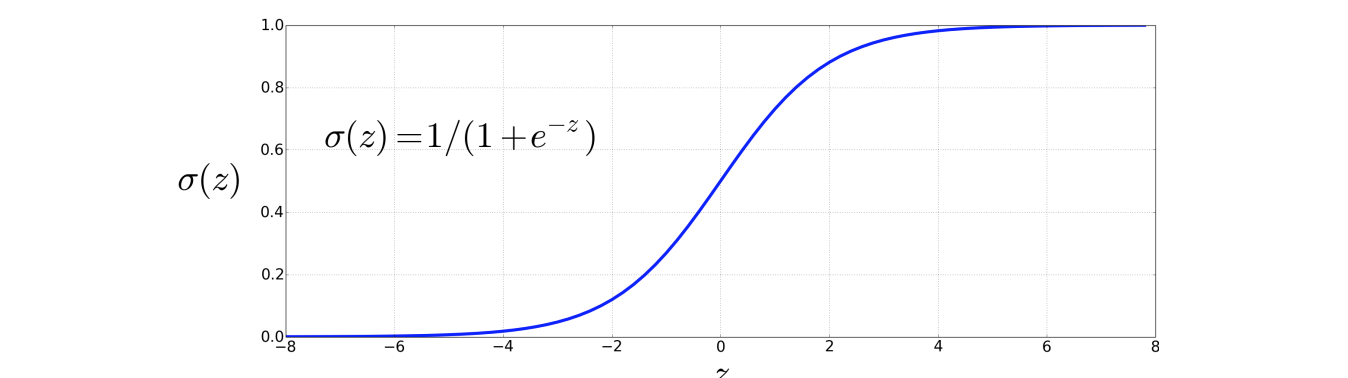
\includegraphics[width=0.7\linewidth]{pic/Klassifikation/sigmoid.png}
\caption{\label{pic:sigmoid} Sigmoid Aktivierungsfunktion}
\end{figure}

Damit der sich ergebende Wert aus $\sigma(z)$ als Wahrscheinlichkeit interpretiert werden kann, muss \begin{equation}
p(y=1) + p(y=0) = 1 \label{Wahrscheinlichkeit} 
\end{equation}
gelten. Dies ist dann der Fall, wenn:
\begin{equation}
p(y=1) =  \frac{1}{1+e^{-z} }  \label{p(y=1)}  
\end{equation}
und
\begin{equation}
p(y=0) =  1 - \frac{1}{1+e^{-z} }  \label{p(y=0)}  
\end{equation}
ist.


\subsubsection{Cross-Entropy Verlustfunktion}
Für den Algorithmus ist der Gesamtfehler geringer, wenn die Klassenwahrscheinlichkeiten eindeutiger sind. Idealerweise gibt es keinen Fehler, wenn: 
\begin{equation}
\sigma(z) =  0 \textrm{ für $y$ = 0 } \label{p(y=0)}  
\end{equation}
und 
\begin{equation}
\sigma(z) =  1 \textrm{ für $y$ = 1 } \label{p(y=0)}  
\end{equation}
vorhergesagt werden. 

Ziel des Algorithmus ist es, den Gesamtfehler möglichst gering zu halten. Dabei wird der Gesamtfehler mit einer Cross-Entropy Verlustfunktion beschrieben. Diese wird anschließend mit dem Gradientenverfahren minimiert. 
Die Cross-Entropy-Verlustfunktion lässt sich aus der Bernoulli-Verteilung herleiten.

Da es sich hierbei um ein binäres Klassifizierungsproblem handelt, kann  $p(y|x)$ mit der Bernoulli-Verteilung beschrieben werden:
\begin{equation}
 p(y|x) =  \hat{y}^y (1-\hat{y})^{1-y}.  \label{bernoulli}  
\end{equation}
Zur einfachen mathematischen Handhabung wird der Ausdruck \ref{bernoulli} logarithmiert:
\begin{equation}
\log p(y|x) =  \log [\hat{y}^y  (1-\hat{y})^{1-y}] = y \log \hat{y} + (1-y) \log (1-\hat{y}).  \label{log bernoulli}  
\end{equation}
Nennen wir die Differenz zwischen der Prognose und der tatsächlichen Klasse mit $L(\hat{y}, y)$, dann lässt sich das Minimierungsproblem wie folgt darstellen:
\begin{equation}
L(\hat{y}, y) =  -\log p(y|x) = - [ y \log \hat{y} + (1-y) \log (1-\hat{y})]. \label{Verlustfunktion}  
\end{equation}

\subsubsection{Gradientenverfahren} \label{subsubsec:Gradientenverfahren}
Wie bereits erwähnt, besteht das Ziel des Gradientenverfahrens darin, einen Gewichten-Vektor $\hat{\theta}$ mit: 
\begin{equation}
\hat{\theta} = \underset{\theta}{\text{argmin}} \frac{1}{m} \sum_{i=1}^{m} L (f(x^{(i)};\theta),y^{(i)}). \label{Gradient}
\end{equation}
zu finden, der den Verlust im Mittel mininiert. Das Minimierungsproblem wird mit dem Gradientenverfahren gelöst.

Die logistische Regression hat im Gradientenverfahren einen wesentlichen Vorteil im Vergleich zu den Multi-Layer Neural Networks (NNs). Da die Verlustfunktion im Gegensatz zu den Multi-Layer NNs konvex ist, existiert ein eindeutiges globales Minimum und es gibt keine lokale Minima, die den Algorithmus beeinträchtigen können.

\begin{figure}[H]
\centering
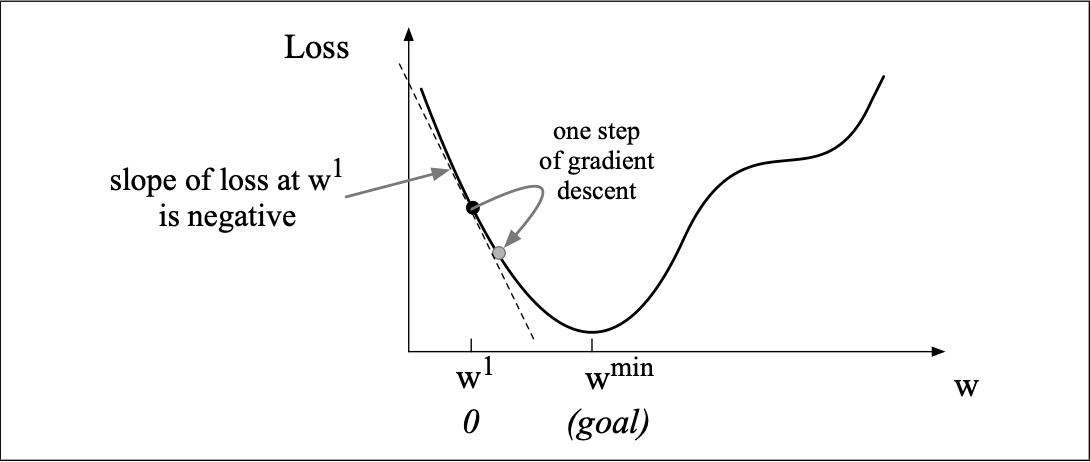
\includegraphics[width=0.5\linewidth]{pic/Klassifikation/MinimumSuche.png}
\caption{\label{pic:MinimumSuche} Iterative Suche nach dem Minimum}
\end{figure}


Basierend auf den Gradientenvektor 
\begin{equation}
\Delta L (f(x;\theta),y) = \begin{bmatrix}  \frac{\delta}{\delta w_{1}} L (f(x;\theta),y) \\ 
 \frac{\delta}{\delta w_{2}} L (f(x;\theta),y) \\ 
. \\ 
. \\ 
. \\ 
  \frac{\delta}{\delta w_{n}} L (f(x;\theta),y) \\ 
   \frac{\delta}{\delta b} L (f(x;\theta),y) \end{bmatrix} \label{Gradientenvektor}
\end{equation}
lassen sich neue Gewichte wie folgt berechnen:
\begin{equation}
\theta_{t+1} = \theta_{t} - \eta \Delta L (f(x;\theta),y),  \label{neue Gewichte}
\end{equation}

wobei $\eta$ die Lernrate entspricht. Diese beschreibt wie schnell den Abhang entlang gefahren wird. Die Wahl von $\eta$ hat einen Einfluss auf die Geschwindigkeit der Suche nach dem Minimum. Ist $\eta$ zu klein gewählt, ist die Laufgeschwindigkeit langsamer und andersrum ist die Laufgeschwindigkeit schneller, wenn $\eta$ groß gewählt ist. Ist jedoch $\eta$ zu groß gesetzt, könnte man das Minimum verpassen. Die Lernrate soll daher optimal gewählt werden, sodass die Laufgeschwindigkeit groß genug ist, um das Minimum schnellstmöglich zu finden und gleichzeitig das System nicht mit unnötig vielen Berechnungen zu belasten.

\begin{figure}[H]
\centering
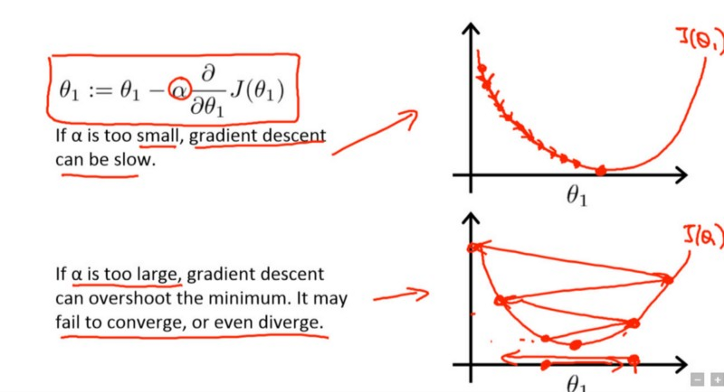
\includegraphics[width=0.5\linewidth]{pic/Klassifikation/Lernrate.png}
\caption{\label{pic:Lernrate} Einfluss der Lernrate auf die Suche nach dem globalen Minimum}
\end{figure}

\subsection{EfficientNet}
\label{EfficientNet}
Die final gewählte Architektur ist ein EfficientNet, dessen Besonderheit gegenüber früheren Neuronalen Netzen es ist, die Parameter der Auflösung (Größe der Eingabebilder), Breite (Anzahl Neuronen je Layer) und Tiefe (Anzahl Layer) des Netzes im optimalen Verhältnis zu skalieren. Die Intuition ist, dass je größer die Auflösung ist, desto breiter und tiefer muss das Netz sein, um dessen Eigenschaften zu repräsentieren, aber eine weitere Verbreiterung und Vertiefung über das Verhältnis hinaus (bei gleichbleibender Auflösung) sinkende Erträge erzielt und somit durch verlangsamtes Training das Gesamtmodell verschlechtert.

Mathematisch ist es ein Optimierungsproblem mit den Parametern Tiefe $d = \alpha^\oslash$, Breite $w = \beta^\oslash$, Auflösung $r = \gamma^\oslash$, sodass $\alpha.\beta^2.\gamma^2 \approx 2$, wobei $\alpha,\beta,\gamma$ mit einem Grid Search Algorithmus bestimmt werden. Die Floating Point Operations Per Second (FLOPS) sind durch $(\alpha.\beta^2.\gamma^2)^\oslash$ berechenbar. Da $\alpha.\beta^2.\gamma^2$ etwa 2 ist, erhöht sich für jedes weitere $\oslash$ die Anzahl der FLOPS um $2^\oslash$. Wenn $\oslash = 1$ ergibt eine GridSearch mit $\alpha.\beta^2.\gamma^2 \approx 2$ die Werte $\alpha = 1.2, \beta = 1.1, \gamma = 1.15$. Dies ist das EfficientNet-B0 Modell. Für die Modelle B1-B7 werden die eben genannten Werte für $\alpha, \beta, \gamma$ nur noch skaliert.

\begin{figure}[H]
\centering
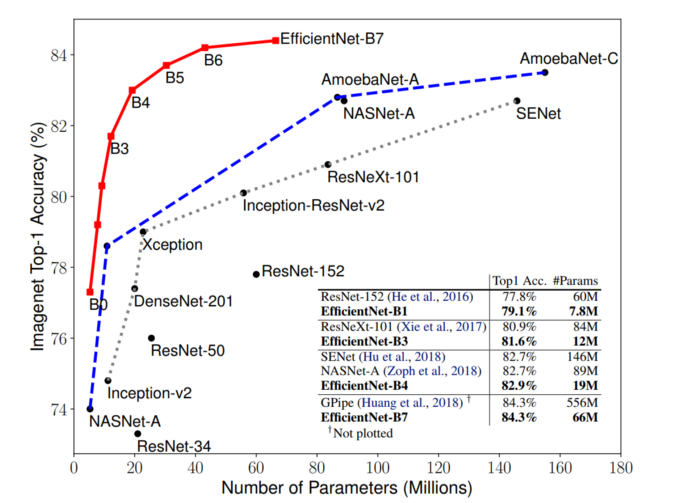
\includegraphics[width=0.5\textwidth]{./pic/Klassifikation/EfficientNetPerformance.png}
\caption{Anzahl Parameter und Performance im Vergleich. \textit{Quelle}: \cite{22}}
\end{figure}

\section{Umsetzung}

Die Umsetzung der Klassifikation geschieht über die Nutzung eines in PyTorch vorimplementierten EfficientNet \cite{22}. Die gewählte Größe unseres EfficientNet ist das größte welches zum Zeitpunkt des Projektes zur Verfügung steht - B7.  Das Netz arbeitet hierbei auf Bildern der Maße 448x448 und ist somit den 509x496 der OCTs der Uniklinik am nächsten. Um die notwendige Auflösung zu erhalten müssen die Ränder der Bilder also beschnitten werden. Dies geschieht ohne erwartete Verluste, da das uns vermittelte Expertenwissen darauf hindeutet dass Ödeme, insbesondere zu behandelnde Ödeme, sich meist zentral auf den Querschnitten befinden.

Desweiteren werden die Bilder vor der Eingabe transformiert, um Kontraste klarer werden zu lassen. Dies passiert indem zunächst die Mittelwerte und Standartabweichungen der RGB Werte des gesamten Datensatzes ermittelt und die RGB Werte der Bilder damit anschließend normalisiert werden, wie zu sehen in Abbildung \ref{pic:Norm}.

Das EfficientNet-B7 wurde auf dem ImageNet Datensatz vortrainiert, welches aus 14.197.122 hochauflösenden Bildern mit 27 Klassen besteht. Dies dient als gute Baseline um Formen und Kanten auf Bildern zu erkennen.

\begin{figure}[H]
\centering
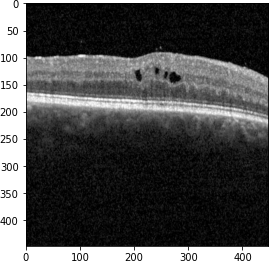
\includegraphics[width=0.25\textwidth]{./pic/Klassifikation/regular_image.png}\hspace{0.5cm}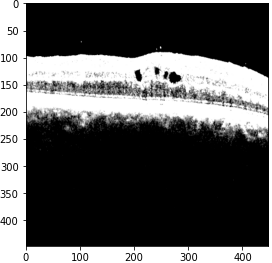
\includegraphics[width=0.25\textwidth]{./pic/Klassifikation/normalized_image.png}
\caption{\label{pic:Norm}Normalisierung der RGB Werte}
\end{figure}

Das letzte Neuron des EfficientNet, welches zur Klassifikation dient, wird mit einem Logistischen Regression Neuron ersetzt, welches ebenfalls auf den Features des vorletzten Layers trainiert wird, um letztlich in die Klassen Ödem und kein Ödem zu klassifizieren. Um die Bedingungen für die Logistische Regression zu optimieren, werden die Features außerdem vor deren Eingabe skaliert.

\begin{figure}[H]
\centering
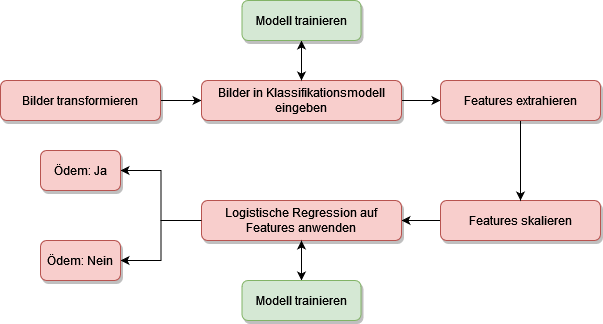
\includegraphics[width=0.7\textwidth]{./pic/Klassifikation/flowchart.png}
\caption{Architektur des Prototypen. - \textit{erstellt mit}: \cite{23}}
\end{figure}

\section{Evaluation}

Zur Evaluation werden zusätzlich zu den extrahierten Features durch das Basis EfficientNet auch die Features nach jeder Finetuning Epoche auf den Trainings- und Testdaten gespeichert, diese mit unterschiedlichen Skalierern skaliert und die jeweiligen skalierten Trainingsfeatures für das Training der Logistischen Regression mit variierenden Hyperparametern verwendet, um dessen Ergebnisse dann mit dem identischen Verfahren auf den Testfeatures zu evaluieren (Abbildung \ref{tab:res1} und \ref{tab:res2}).

Die Evaluation geschieht dann auf den Metriken (Abbildung \ref{tab:Metr}) der Sensitivity und Specificity, mit einer höheren Wertlegung auf die Sensitivity, da die Klassifikation ein Vorfilter für die Segmentierung darstellen sollte, sowie die gesamte Makulaerkennung einen Vorfilter für die Experteneinschätzung der Ärzte, wobei es bei einem Vorfilter viel kritischer ist einen kranken Patienten als gesund zu deklarieren als umgekehrt.

Desweiteren ist es notwendig einen Threshold für die Klassifikation der Logistischen Regression zu bestimmen, tendierend wieder zum Sensitivity bevorzugenden Wertebereich $[0, 0.5]$.

\begin{figure}[H]
\centering
\begin{tabular}{cc c cc}
\multicolumn{2}{c}{\textbf{Treffsicherheit (Klassen)}} && \multicolumn{2}{c}{\textbf{Relevanz (Positive)}} \\
sensitivity: & $\frac{tp}{tp+fn}$ && precision: & $\frac{tp}{tp+fp}$ \\
specificity: & $\frac{tn}{fp+tn}$ && recall: & $\frac{tp}{tp+fn}$
\end{tabular} \\\vspace{0.1cm}
{\footnotesize tp = True Positives, tn = True Negatives, fp = False Positives, fn = False Negatives}
\caption{\label{tab:Metr}Bei der Evaluation verwendete Metriken}
\end{figure}

\begin{figure}[H]
\centering
\begin{tabular}{c|c|c|c|c}
\textbf{epoch} & \textbf{threshold} & \textbf{sensitivity} & \textbf{specificity} & \textbf{sensitivity+specificity} \\\hline\hline
0 & 0.3 & 0.88 & 0.80 & 1.68 \\
0 & 0.4 & 0.83 & 0.85 & 1.68 \\
1 & 0.2 & 0.89 & 0.81 & 1.71 \\
1 & 0.3 & 0.86 & 0.86 & 1.72 \\
1 & 0.4 & 0.85 & 0.88 & 1.73 \\
1 & 0.5 & 0.83 & 0.90 & 1.73 \\
1 & 0.6 & 0.81 & 0.91 & 1.72 \\
\textcolor{red}{2} & \textcolor{red}{0.2} & \textcolor{red}{0.91} & \textcolor{red}{0.83} & \textcolor{red}{1.74} \\
2 & 0.3 & 0.88 & 0.87 & 1.75 \\
2 & 0.4 & 0.86 & 0.89 & 1.75 \\
2 & 0.5 & 0.84 & 0.90 & 1.74 \\
2 & 0.6 & 0.82 & 0.91 & 1.72 \\
3 & 0.3 & 0.86 & 0.86 & 1.72 \\
3 & 0.4 & 0.84 & 0.88 & 1.72 \\
3 & 0.5 & 0.82 & 0.90 & 1.71 \\
4 & 0.2 & 0.90 & 0.84 & 1.73 \\
4 & 0.3 & 0.87 & 0.88 & 1.75 \\
4 & 0.4 & 0.85 & 0.89 & 1.74 \\
4 & 0.5 & 0.82 & 0.91 & 1.73 \\
5 & 0.2 & 0.87 & 0.81 & 1.68 \\
5 & 0.3 & 0.83 & 0.87 & 1.70 \\
6 & 0.2 & 0.85 & 0.84 & 1.69 \\
6 & 0.3 & 0.82 & 0.89 & 1.71 \\
7 & 0.2 & 0.82 & 0.87 & 1.69 \\
8 & 0.2 & 0.83 & 0.83 & 1.66
\end{tabular}
\caption{\label{tab:res1}Klassifikatoren mit sowohl Sensitivity als auch Specificity >= 0.8, \\ Addition der Metriken nur zur Erleichterung eines Vergleichs, der gewählte Favorit in rot}
\end{figure}

\begin{figure}[H]
\begin{tabular}{c|c|c|c|c|c|c}
\textbf{epoch} & \textbf{scaler} & \textbf{solver} & \textbf{threshold} & \textbf{sensitivity} & \textbf{specificity} & \textbf{sensitivity+specificity} \\\hline\hline
1 & StandartScaler & newton-cg & 0.2 & 0.90 & 0.81 & 1.71 \\
1 & StandartScaler & lbfgs & 0.2 & 0.90 & 0.82 & 1.72 \\
1 & StandartScaler & liblinear & 0.2 & 0.90 & 0.82 & 1.72 \\
1 & RobustScaler & lbfgs & 0.2 & 0.91 & 0.80 & 1.71 \\
2 & StandartScaler & newton-cg & 0.2 & 0.91 & 0.82 & 1.74 \\
2 & StandartScaler & lbfgs & 0.2 & 0.91 & 0.82 & 1.74 \\
2 & StandartScaler & liblinear & 0.2 & 0.91 & 0.82 & 1.74 \\
2 & StandartScaler & sag & 0.2 & 0.91 & 0.82 & 1.73 \\
2 & StandartScaler & saga & 0.2 & 0.91 & 0.82 & 1.73 \\
2 & RobustScaler & newton-cg & 0.2 & 0.92 & 0.81 & 1.73 \\
\textcolor{red}{2} & \textcolor{red}{RobustScaler} & \textcolor{red}{liblinear} & \textcolor{red}{0.2} & \textcolor{red}{0.93} & \textcolor{red}{0.82} & \textcolor{red}{1.75} \\
2 & RobustScaler & liblinear & 0.3 & 0.91 & 0.85 & 1.76 \\
3 & StandartScaler & newton-cg & 0.2 & 0.90 & 0.80 & 1.71 \\
3 & StandartScaler & lbfgs & 0.2 & 0.90 & 0.80 & 1.71 \\
3 & StandartScaler & liblinear & 0.2 & 0.90 & 0.80 & 1.71
\end{tabular}
\caption{\label{tab:res2}
Variierende Skalierer und Solver für die Logistische Regression, Klassifikatoren mit Sensitivity >= 0.9 und Specificity >= 0.8, Addition der Metriken nur zur Erleichterung eines Vergleichs, unser gewählter Favorit in rot}
\end{figure}

Die Performance des Favoriten mit Skalierer und angepasstem Solver werden nun noch in Hinsicht der Precision und Recall (=Sensitivity) Werte analysiert (siehe Abbildung \ref{pic:Eval}).

\begin{figure}[H]
\label{pic:Eval}
\centering
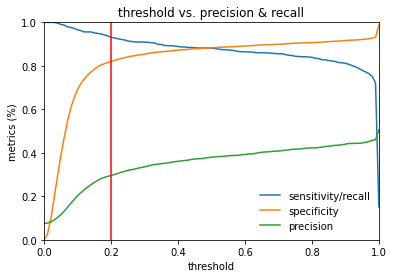
\includegraphics[width=0.7\textwidth]{./pic/Klassifikation/eval.png}
\caption{Performance nach Threshold}
\end{figure}

Wie man sehen kann flacht das Wachstum der Specificity und Precision bei etwa einem Threshold von 0.2 ab, während Sensitity/Recall stetig abnimmt. Dies bestätigt erneut den gewählten Threshold, um Sensitivity/Recall so hoch wie möglich zu halten, ohne alles willkürlich als positiv zu deklarieren.

\textbf{Sensitivity}: 0.98, \textbf{Specificity}: 0.82; \textbf{Precision}: 0.3, \textbf{Recall}: 0.98

Ein Precision Wert von 0.3 wirkt besonders gering, ist jedoch bei einem Klassenunverhältnis wie diesem zu erwarten, da sehr viele negative Bilder die Chance haben, fälschlicherweise als positiv deklariert zu werden und die Precision das Verhältnis an wirklich positiven gegenüber wirklich negativen der als positiv vorhergesagten Bilder beschreibt.